\documentclass[11pt]{article}

% Accepted camera-ready working copy. The submitted review version remains main.tex.
\usepackage{acl}

\usepackage[T1]{fontenc}
\usepackage[utf8]{inputenc}
\usepackage{lmodern}
\usepackage{inconsolata}
\usepackage{graphicx}
\usepackage{booktabs}
\usepackage{amsmath}
\usepackage{amssymb}
\usepackage{xcolor}
\graphicspath{{../figures/}}

\newcommand{\rcps}{\textnormal{\textsc{RCPS}}}

\title{Retrieval-Conditional Parsing Score (RCPS):\\Choosing Document Parsers by Retrieval, Not by Appearance}

% Author order is frozen to OpenReview Submission #384. Do not reorder.
\author{
  \textbf{Sang-Woo Son},
  \textbf{Hyeong-seob Kim},
  \textbf{Hyeonsang Kim},\\
  \textbf{Hyun-woo Cho},
  \textbf{Jinmo Kim}
}
% CAMERA-READY METADATA PENDING: verify affiliations and author emails against
% OpenReview. The Industry Track Chairs have been asked whether Hyeong-seob Kim
% may be identified as corresponding author without changing this author order;
% add the ACL-template Correspondence line only after their written reply.

\begin{document}
\maketitle

\begin{abstract}
Document parsers are often selected with intrinsic measures of transcription fidelity and boundary quality, even though their outputs ultimately serve retrieval. We show that this mismatch can alter which parser a team would deploy. In the submitted-output analysis, MinerU-off has one of the highest Boundary Clarity scores in our candidate pool. In a separate table-enabled audit, Prod attains a Hit@1 of $0.549$, compared with $0.123$ for MinerU-on---a difference of $42.6$ percentage points; Prod's value is $4.47\times$ as high. We define the Retrieval-Conditional Parsing Score (\rcps{}), a training-free protocol for ranking parser--chunker combinations on a held-out question--answer (Q--A) retrieval probe. \rcps{} averages MRR at cutoffs 1, 5, and 10 across specified retrievers under a shared format-normalised exact-span relevance rule. A retriever-free coverage diagnostic distinguishes reference spans with no exact match in parser output from spans divided by chunk boundaries. Under this rule, $20.2\%$ of reference spans have no match in Prod's output, whereas at most $2.3\%$ are split. Within our candidate pools, the \rcps{} range across parsers evaluated on 294 pages is $0.447$, compared with $0.058$ across chunkers. On source-aligned OHR-Bench data, semantic noise reduces retrieval while Boundary Clarity remains stable or changes non-monotonically. On an audited six-domain compatibility subset, two direct preference optimization checkpoints have Hit@5 estimates $0.95$ and $1.15$ percentage points above Prod. We release KoGovDoc-RAG evaluation files and an \rcps{} reference implementation.
\end{abstract}

\section{Introduction}

\begin{figure*}[t]
\centering
% CAMERA-READY FIGURE BLOCKER (deferred until the final visual pass): establish
% one canonical source before regeneration. The current export still shows
% table-off MinerU and unsupported Distill values, omits the 229+65 page /
% 527+136 Q--A composition, and is too small at 0.70 width.
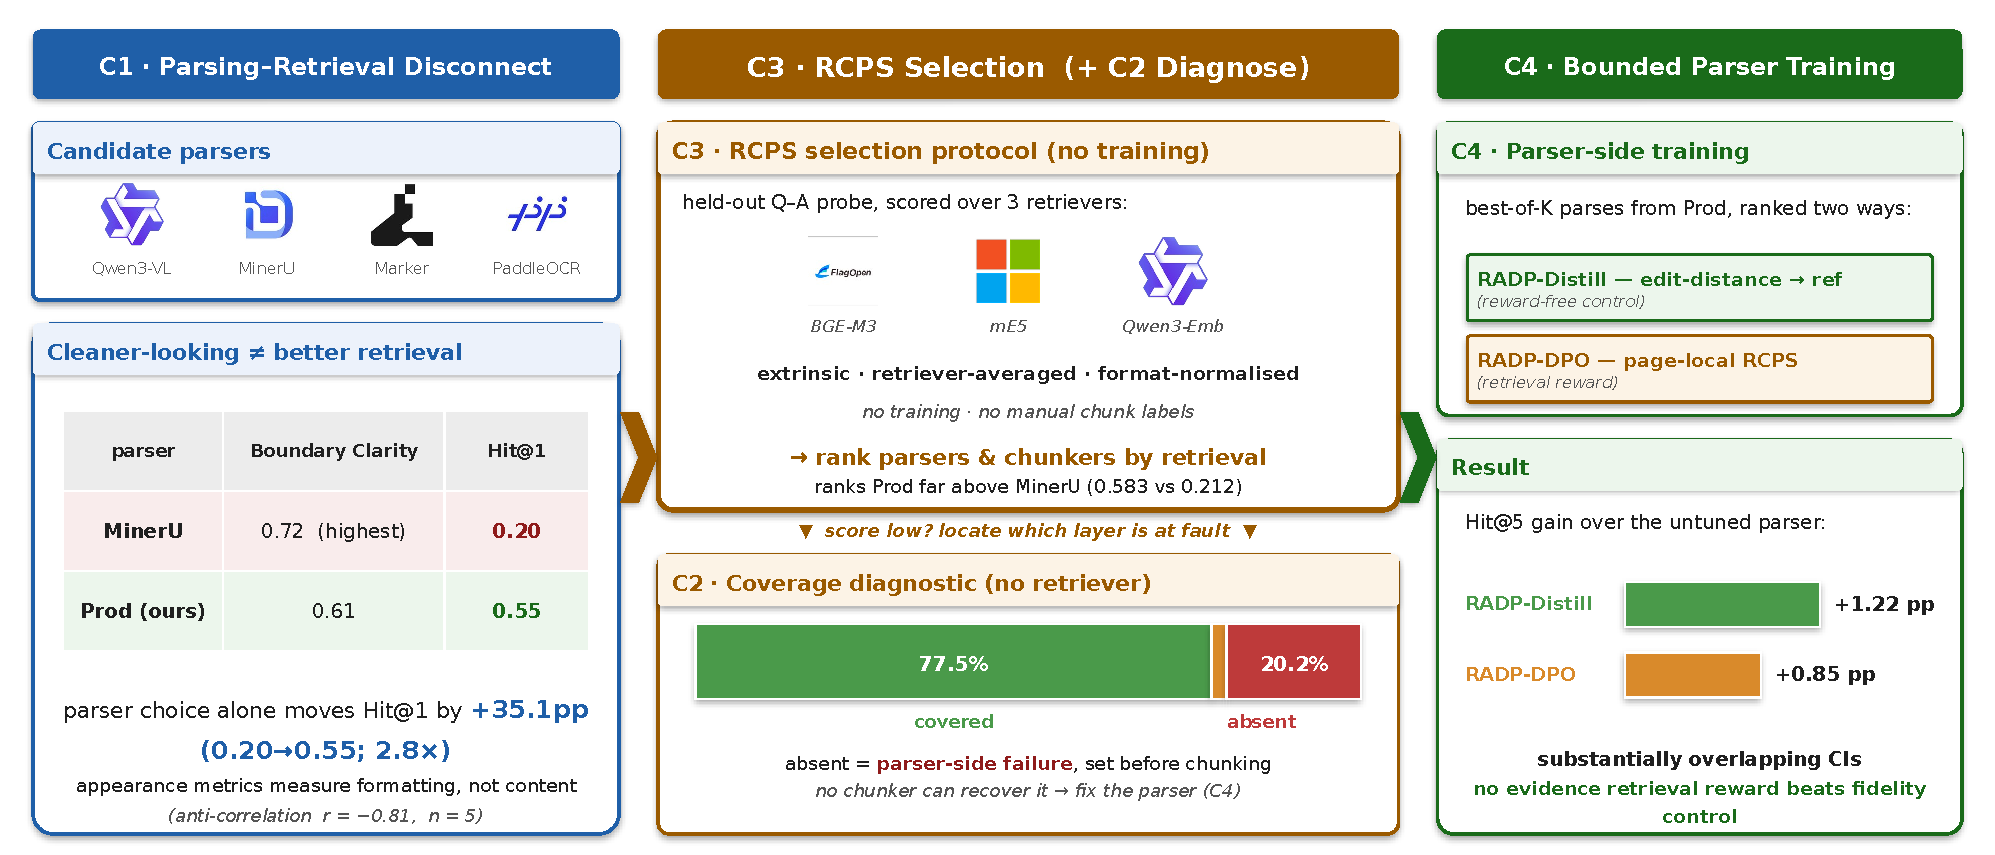
\includegraphics[width=0.70\textwidth]{fig_overview.pdf}
\caption{\textbf{Overview.} Intrinsic boundary metrics can misrank parsers. A retriever-free diagnostic distinguishes exact-span absence in parser output from chunk-boundary splitting, while \rcps{} ranks parser--chunker combinations on a held-out Q--A probe. We then assess whether parser-side training provides additional retrieval gains.}
\label{fig:overview}
\end{figure*}

Retrieval-augmented generation (RAG) systems for documents often begin with scanned or born-digital PDFs. A parser converts each page to text before chunking, embedding, and retrieval, so omitted or corrupted content can limit downstream retrieval. Parsers therefore ought to be evaluated by the retrieval they enable. In practice, however, teams commonly choose among them using intrinsic measures such as edit distance to a reference transcription or Boundary Clarity (BC) \citep{zhao2025moc}. These measures capture reference fidelity or boundary structure, but neither directly measures retrievability.

We encountered this mismatch while building a production RAG system for Korean government documents. In the submitted-output analysis, MinerU-off \citep{mineru2025} combines a high BC score ($0.716$) with a low Hit@1 ($0.197$). A separate table-enabled audit gives MinerU-on a Hit@1 of $0.123$, compared with $0.549$ for Prod---a $42.6$ percentage-point gap, with Prod $4.47\times$ as high. Because the two MinerU runs also differ in their software and retrieval environments, we do not treat them as a causal table-recognition ablation. On source-aligned OHR-Bench data \citep{zhang2024ohr}, controlled semantic corruption likewise reduces retrieval while BC remains nearly fixed or changes non-monotonically.

Two additional findings clarify what to do after parser selection. On Prod output, $20.2\%$ of reference spans have no normalised exact match before chunking, whereas at most $2.3\%$ are split by one of the tested chunkers. Separately, on a six-domain OHR-Bench compatibility subset, two audited RADP-DPO checkpoints have Hit@5 estimates approximately one percentage point above Prod. Because this experiment uses a different dataset and endpoint, we do not compare its effect size directly with the parser-selection difference.

\paragraph{Contributions.} Our contributions are fourfold. First, we document a mismatch between intrinsic parsing metrics and retrieval (C1). Second, we introduce a retriever-free diagnostic that separates reference spans absent from parser output from spans divided by chunk boundaries (C2). Third, we define \rcps{}, a training-free protocol for ranking parsers and chunkers on a held-out retrieval probe (C3). Finally, we estimate retrieval differences associated with retrieval-aware parser training and quantify their uncertainty (C4). Our primary scope is answer-span retrievability, not generated-answer quality. Appendix~\ref{app:e2e} provides a limited three-parser check of whether the top-ranked parser also performs best in end-to-end answering.

The repository contains the frozen \textbf{KoGovDoc-RAG} evaluation files---663 question--answer pairs over 294 pages---and a reference implementation of \rcps{}.\footnote{\url{https://github.com/wigtn/WigtnOCR-RADP}}

\section{Related Work}

\paragraph{Prior evidence.} OHR-Bench \citep{zhang2024ohr} measures how optical character recognition (OCR) noise propagates through RAG, while EnterpriseDocBench \citep{enterprisedocbench2026} and concurrent studies \citep{goodocr2026,song2026ocr} report weak associations between parsing quality and retrieval. Most parsing benchmarks still rank systems by intrinsic fidelity \citep{ouyang2025omnidocbench}. Vision-based retrieval \citep{faysse2024colpali} avoids text parsing altogether and is therefore complementary to the text pipelines studied here. We are unaware of prior work that combines a reusable parser-selection protocol with a diagnostic that separates spans missing from parser output from spans divided by chunk boundaries.

\paragraph{Training.} Retrieval-oriented training has been applied to chunking \citep{jina2024late,duarte2024lumber,zhao2024meta,zhao2025moc,singh2024chunkrag}, embedding models \citep{conti2025insent,zhao2025lmar}, and retriever or reader components \citep{nguyen2024rewardrag,chia2025mlongdoc,yan2025rpo}. These interventions target downstream layers: M-LongDoc \citep{chia2025mlongdoc} makes a reader robust to retrieved context, whereas InSeNT \citep{conti2025insent} trains contextual embeddings. Parser training has instead used edit-distance and layout rewards \citep{infinity_parser} or query guidance for efficient RAG \citep{agenticocr}. We intervene at the earlier parser layer by testing a retrieval reward and designing a fidelity-based control. Because aligned per-Q--A results for the control are unavailable, C4 does not report a matched quantitative comparison. Our main contributions (C1--C3) require no training.

\section{Two Tools: Selection and Diagnosis}

\subsection{\rcps{}: Retrieval-Conditional Parsing Score}
\label{sec:rcps}

\rcps{} ranks parsers by the retrieval performance enabled by their outputs rather than by visual or formatting quality. It is an evaluation protocol built from standard truncated mean reciprocal rank (MRR), not a new similarity function. The protocol has three design choices. First, it is \emph{extrinsic}: candidates are evaluated on a held-out Q--A probe over the parsed corpus. Second, it is \emph{retriever-averaged}: scores are averaged across a specified set of retrievers to reduce dependence on any single one. Here, a retriever is the shared nearest-neighbour search pipeline instantiated with a particular embedder. Third, the protocol uses \emph{format-normalised exact-span relevance}: a chunk is relevant only when it comes from the reference page and contains the reference answer after shared whitespace and Markdown normalisation. We use \rcps{} \emph{score} for the aggregate in Equation~\ref{eq:rcps} and \rcps{} \emph{protocol} for this complete procedure.

Given a parser $P$, a chunker $C$, a Q--A set $D = \{(q_i, a_i, \text{page}_i)\}$, a set of retrievers $R$, and cutoffs $K$, \rcps{} averages MRR over all retriever--cutoff pairs:
\begin{equation}
\label{eq:rcps}
\begin{aligned}
\text{RCPS}(P,C)
  &= \frac{1}{|R|\,|K|} \sum_{r \in R} \sum_{k \in K} \\
  &\quad \text{MRR}@k(r, C(P), D).
\end{aligned}
\end{equation}
Here, $C(P)$ denotes the corpus obtained by parsing with $P$ and then chunking with $C$. We instantiate $R$ with BGE-M3 \citep{chen2024bgem3}, multilingual-e5-large \citep{wang2024me5}, and Qwen3-Embedding-8B \citep{qwen3emb}, and use $K = \{1,5,10\}$. Averaging over cutoffs avoids tying selection to one retrieval depth. Figure~\ref{fig:protocol} shows the workflow.

\begin{figure}[t]
\centering
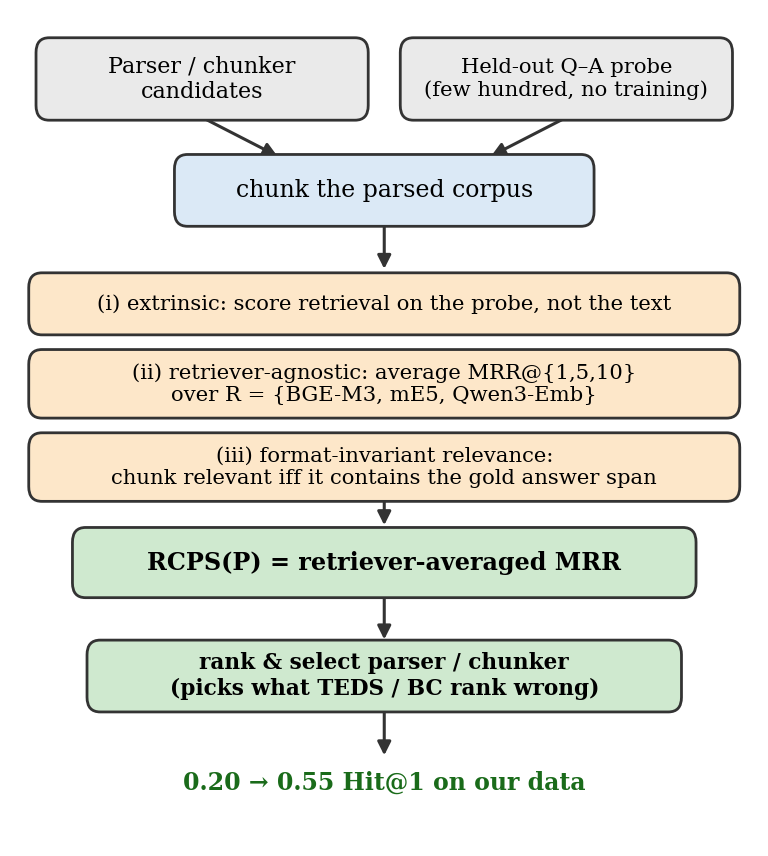
\includegraphics[width=0.6\columnwidth]{fig_rcps_protocol.png}
\caption{\rcps{} wraps standard MRR with a held-out Q--A probe, retriever averaging, and format-normalised relevance. The resulting score ranks candidate parsers and chunkers without requiring additional training as part of evaluation.}
\label{fig:protocol}
\end{figure}

\paragraph{Execution.} First, construct a representative held-out Q--A probe whose answer spans occur verbatim in its reference pages. Our probe is model-generated; an LLM-based quality check accepted 94 of a 100-pair sample (\S\ref{sec:setup}). Each parser candidate processes the evaluation pages once. Every resulting corpus is then chunked, indexed, and searched with each retriever. For $m$ parsers, $c$ chunkers, and $|R|$ retrievers, the protocol requires $m$ parsing runs and $mc|R|$ indexing-and-retrieval evaluations.

\paragraph{Interpretation.} Equation~\ref{eq:rcps} yields a ranking that can inform deployment. The protocol requires neither model training nor manual chunk-level relevance labels, because relevance follows from the reference span and source page. Fixing $C$ ranks parsers; fixing $P$ ranks chunkers. The score is meaningful only relative to the candidate pool and probe.

\subsection{Coverage Diagnostic: Parser or Chunker?}
\label{sec:coverage}

A low \rcps{} value does not reveal whether the parser, chunker, or retriever caused the failure. We isolate the first two stages with a retriever-free diagnostic. With parser output fixed, each reference answer is \emph{covered} if its normalised span appears in full within at least one chunk. It is \emph{split} if the span exists in the source-page transcription but no individual chunk contains it in full, and \emph{absent} if that page output contains no normalised exact match. A split case is a boundary-induced match failure that overlap may repair. An absent case indicates that rechunking alone cannot restore an exact-span match. These labels are operational: \emph{absent} does not by itself prove semantic omission. The split--absent breakdown therefore indicates which stage to inspect first.

\begin{figure}[!t]
\centering
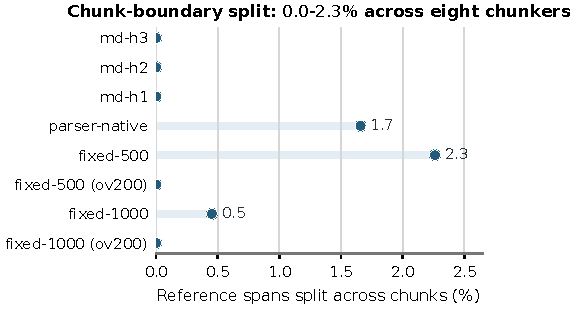
\includegraphics[width=0.70\columnwidth]{fig_coverage.pdf}
\caption{Coverage diagnostic with the parser fixed to Prod. The absent rate ($20.2\%$) is measured before chunking and is therefore constant; changing the chunker affects only the split rate, which reaches at most $2.3\%$.}
\label{fig:coverage}
\end{figure}

\section{Experiments}

\subsection{Setup}
\label{sec:setup}

\paragraph{Datasets.} \textbf{KoGovDoc-RAG} contains 663 Q--A pairs over 294 evaluation pages: 229 Korean government pages and 65 arXiv pages. Qwen3-VL-30B first produced reference Markdown, which we manually de-noised. We then used \texttt{gpt-5.4-2026-03-05} to generate Q--A pairs from those references; an LLM-based quality check accepted 94 of a 100-pair sample. Parser training instead uses a separate 2{,}667-page Prod corpus containing 6{,}164 generated Q--A. Cross-domain experiments use two source-page-aligned OHR-Bench subsets \citep{zhang2024ohr}: 1{,}043 Law--Manual Q--A for controlled perturbations and a 2{,}036-Q--A, six-domain compatibility subset for the audited parser-training evaluation. Appendix~\ref{app:noise} explains the version-alignment audit and exclusions.

\paragraph{Parsers and evaluation folds.} \textbf{Prod} is our production parser, a Qwen3-VL-2B model \citep{qwen3vl} fine-tuned for Korean document parsing; all training deltas use it as the baseline. RADP-aux is evaluated on a 73-page fold containing 202 Q--A. RADP-DPO, the reference-free Simple Preference Optimization (SimPO) control, and the mechanism analysis are evaluated on all 663 Q--A, whose evidence occurs on 242 of the 294 evaluation pages. Retrieval indexes all 294 pages, so the remaining 52 pages serve as distractors. No evaluation page or Q--A is used to construct training preferences: all candidates and preferences come from the separate, page-disjoint 2{,}667-page training corpus.

For MinerU, \emph{MinerU-off} denotes the submitted output without table recognition, while \emph{MinerU-on} denotes the later audited, table-enabled output. Correlation analyses use MinerU-off; deployment comparisons use MinerU-on. We do not combine the two configurations in one correlation.

\paragraph{Training and evaluation.} Evaluation parses from trained checkpoints are decoded deterministically (temperature 0, maximum 1{,}536 tokens); the stochastic candidate sampling used to construct preferences is described in Appendix~\ref{app:milestones}. We fine-tune with Low-Rank Adaptation (LoRA) \citep{hu2021lora} ($r=8$, $\alpha=32$) and sweep $\lambda\in\{0,0.1,0.3,0.5\}$ for RADP-aux. \rcps{} uses the retrievers and cutoffs defined in \S\ref{sec:rcps}. Unless stated otherwise, confidence intervals (CIs) are paired 95\% percentile-bootstrap intervals with 1{,}000 resamples, preserving Q--A pairing across systems.

\subsection{Parsing--Retrieval Disconnect and Coverage (C1--C2)}
\label{sec:c1c2}

\paragraph{KoGovDoc-RAG (Figure~\ref{fig:disconnect}; Table~\ref{tab:grid}).} Across the five deployment configurations with complete 294-page outputs, \rcps{} ranges from $0.137$ to $0.584$: vision--language parsers rank highest and OCR systems trail. MinerU-off is reported separately for the submitted-output diagnostics and correlations. Marker is available only on a 38-page subset, where it scores $0.073$, so we exclude it from complete-output comparisons. Most of the spread comes from the OCR-style parsers rather than the near-tied vision--language configurations. The Qwen3-VL-30B teacher and Prod have the two highest aggregate scores, $0.584$ and $0.583$, respectively.

The intrinsic-metric analysis uses MinerU-off. Among the four parsers evaluated on all 294 pages and with defined BC \citep{zhao2025moc}, the Pearson correlation between BC and \rcps{} is $r=-0.74$. Adding Marker's 38-page result changes the estimate to $r=-0.81$ ($n=5$); PaddleOCR is excluded because its BC is undefined. MinerU-off and Marker have the highest BC values ($\approx0.72$) but rank near the bottom on retrieval. Because the samples contain only four or five parsers and Marker uses a smaller page set, both correlations are descriptive.

\begin{figure*}[t]
\centering
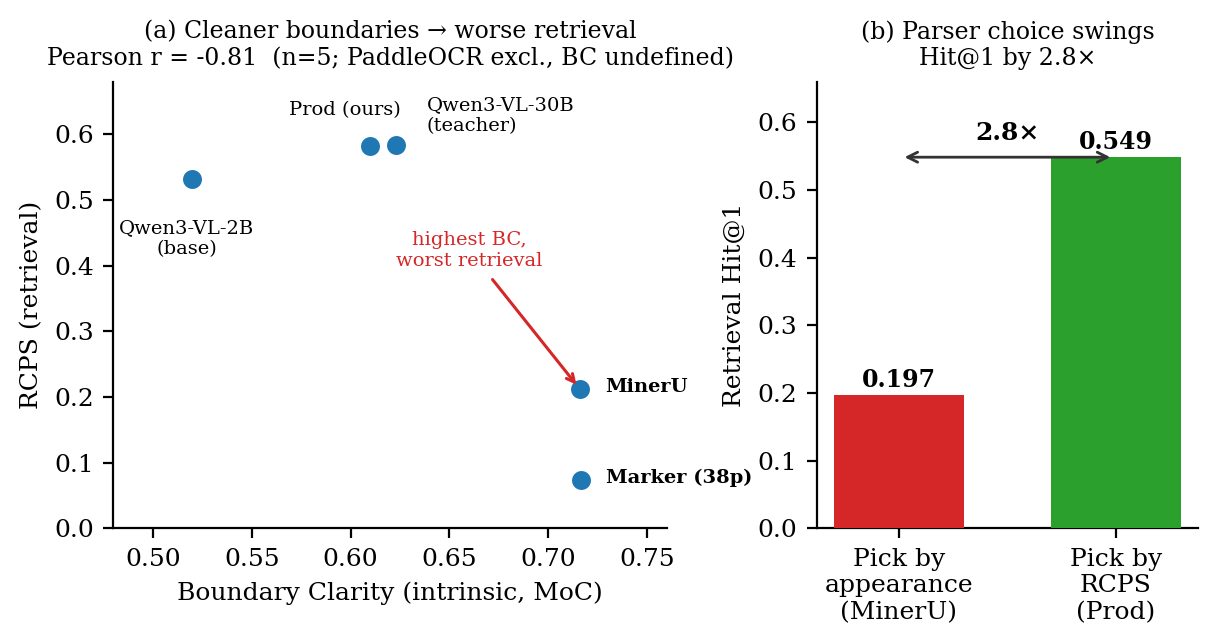
\includegraphics[width=0.56\textwidth]{fig_disconnect.png}
\caption{Parsing--retrieval mismatch on KoGovDoc-RAG. (a) With MinerU-off, BC and \rcps{} are negatively correlated ($r=-0.81$, $n=5$; PaddleOCR excluded because BC is undefined). Marker uses 38 pages; excluding it gives $r=-0.74$ ($n=4$). (b) In the separately audited MinerU-on comparison, Prod exceeds MinerU-on Hit@1 by $42.6$ percentage points ($0.549$ vs.\ $0.123$; $4.47\times$).}
\label{fig:disconnect}
\end{figure*}

\paragraph{Cross-domain sensitivity test.} We evaluate three benchmark parser outputs and twelve controlled perturbations---not fifteen independent parsers---on the source-aligned Law--Manual subset of OHR-Bench (1{,}043 Q--A; Appendix~\ref{app:noise}). Across the available perturbation severities, semantic noise reduces \rcps{} within every family, but BC responds inconsistently. For MinerU, BC remains between $0.628$ and $0.657$ while \rcps{} falls from $0.595$ to $0.265$ ($55\%$). For Qwen2.5-VL, BC stays near $0.563$ while \rcps{} falls by $9\%$. For GOT, BC rises from $0.586$ to $0.624$ while \rcps{} falls from $0.461$ to $0.298$.

We make no claim beyond the aligned Law--Manual subset. Appendix~\ref{app:noise} reports the descriptive aggregate correlation across variants.

\paragraph{Diagnosing exact-span loss (Figure~\ref{fig:coverage}).} The metric mismatch does not identify the responsible pipeline stage. On Prod's full output (294 pages, 663 Q--A), the retriever-free diagnostic marks $20.2\%$ of answers absent. Depending on the tested chunker, at most $2.3\%$ are split. Thus, for roughly one answer in five, rechunking the fixed Prod output cannot recover a normalised exact-span match. This diagnostic complements \rcps{} selection by showing when changing the chunker is insufficient.

The MinerU-off diagnostic gives a $70.4\%$ absent rate, compared with $20.2\%$ for Prod. The MinerU--Prod gap remains between $50.2$ and $51.7$ percentage points under exact-span matching, an OCR-tolerant matcher, and a GPT-5.4 recoverability judge (Appendix~\ref{app:familyneutral}). Limitations reports the separate MinerU-on audit.

\subsection{\rcps{} Selects Both Parsers and Chunkers (C3)}
\label{sec:c3}

\begin{table}[!b]
\centering\footnotesize
\setlength{\tabcolsep}{2.5pt}
\begin{tabular}{lcccc}
\toprule
Parser & BC & CS & \rcps{} & Hit@1 \\
\midrule
\multicolumn{5}{l}{\textit{Deployment comparison (294 pages)}} \\
Qwen3-VL-30B (teacher) & 0.623 & 3.38 & \textbf{0.584} & 0.545 \\
Prod (ours, 2B) & 0.610 & 3.07 & 0.583 & 0.549 \\
Qwen3-VL-2B (base) & 0.520 & 3.74 & 0.532 & 0.500 \\
PaddleOCR & --- & 3.46 & 0.140 & 0.125 \\
MinerU-on & --- & --- & 0.137 & 0.123 \\
\addlinespace
\multicolumn{5}{l}{\textit{Submitted-output diagnostic (294 pages)}} \\
MinerU-off & 0.716 & 2.81 & 0.212 & 0.197 \\
\addlinespace
\multicolumn{5}{l}{\textit{Partial output}} \\
Marker (38p) & \textbf{0.717} & 3.41 & 0.073 & 0.068 \\
\bottomrule
\end{tabular}
\caption{KoGovDoc-RAG parser results, with \rcps{} averaged across three retrievers and $k\in\{1,5,10\}$. BC is Boundary Clarity (higher is better); CS is Chunk Stickiness (lower is better). Deployment rows use MinerU-on, while correlations use the separately shown MinerU-off. Marker is excluded from complete-output comparisons.}
\label{tab:grid}
\end{table}

\paragraph{Selecting parsers.} The deployment block of Table~\ref{tab:grid} gives the \rcps{} ranking. In the separately audited MinerU-on comparison, Prod attains $0.583$ \rcps{} and $0.549$ Hit@1, whereas MinerU-on attains $0.137$ and $0.123$, respectively; Prod's Hit@1 is therefore $4.47\times$ as high. The Qwen3-VL-30B teacher and Prod differ by only $0.001$ \rcps{} at the reported precision. Because the complete parser grid lacks paired uncertainty estimates, we treat them as descriptively near-tied rather than claim equivalence. Latency and compute may therefore inform deployment alongside retrieval quality.

\paragraph{Selecting chunkers.} With Prod fixed, the same probe ranks four strategies: Markdown heading depth 3 (md-h3, $0.593$) $>$ parser-native boundaries ($0.583$) $>$ LumberChunker \citep{duarte2024lumber} ($0.557$) $>$ fixed 500-character windows ($0.535$). These results show that the same held-out probe can select among chunkers once the parser is fixed. Across the four chunkers, the \rcps{} range is $0.058$. The heterogeneous parser pool spans a much larger $0.447$, although the range among only the three vision--language parsers is similar to the chunker range ($0.052$).

\paragraph{Why average over retrievers?} Table~\ref{tab:ablation} compares BGE-M3 alone with the full three-retriever protocol on five complete-output configurations, with MinerU represented by MinerU-off. The rankings differ only in the nearly tied 30B--Prod pair (Kendall $\tau=0.80$). Averaging therefore reduces reliance on one embedder in this candidate pool, but we do not claim a broad reversal. If the deployment retriever is fixed, teams can score with that retriever; averaging is a hedge when the retriever is undecided or candidates are nearly tied. BGE-M3 leaves the four-chunker ordering unchanged. A separate aggregate-only audit of the same MinerU-off parser grid shows that replacing the average over $k\in\{1,5,10\}$ with three-retriever MRR@10 preserves both the five-parser and four-chunker orders ($\tau=1.0$). Because aligned per-Q--A results are unavailable for the complete grid, this check does not measure probe-resampling stability.

\begin{center}
\begin{minipage}{\columnwidth}
\centering\footnotesize
\captionsetup{hypcap=false}
\setlength{\tabcolsep}{3pt}
\begin{tabular}{lcc}
\toprule
Protocol configuration & Top pair & $\tau$ vs \rcps{} \\
\midrule
BGE-M3 only & Prod $\succ$ 30B & 0.80 \\
full \rcps{} & 30B $\succ$ Prod & --- \\
\bottomrule
\end{tabular}
\captionof{table}{Retriever-averaging ablation on five complete-output configurations, with MinerU represented by MinerU-off and Marker excluded. Both rows use the same format-normalised relevance rule. Only the top pair changes; lower ranks are unchanged. ``30B'' denotes the Qwen3-VL-30B teacher.}
\label{tab:ablation}
\end{minipage}
\end{center}

\subsection{Parser-Side Training Results (C4)}
\label{sec:c4}\label{sec:mechanism}

Because some exact spans are already absent before chunking, we ask whether parser training can help after selection. We study the two RADP methods introduced in \S\ref{sec:setup}: the hidden-state auxiliary loss RADP-aux and RADP-DPO with a page-local BGE-M3 retrieval reward \citep{rafailov2023dpo}. The pre-specified pilot criterion required an \rcps{} gain of at least 5 percentage points with a 95\% confidence-interval lower bound above zero. Neither RADP-aux nor any evaluated RADP-DPO checkpoint met this criterion. Appendix~\ref{app:dpo} provides the results and the reference-free SimPO control \citep{meng2024simpo}. RADP-Distill is a fidelity-based control that ranks candidates by edit distance to reference Markdown and uses no retrieval reward. Its aligned per-Q--A results are unavailable, so we exclude it from the quantitative comparison.

RADP-DPO R2 is a warm-started preference-training round, whereas R3 expands the candidate pool and adds full-corpus hard negatives (Appendix~\ref{app:milestones}). Starting from a 2{,}264-pair legacy artifact, we exclude 228 Q--A whose source-page identifiers do not align with the current parser-output bundle. This leaves a 2{,}036-Q--A compatibility subset across six domains. On this subset, R2 and R3 have Hit@5 values $0.95$ and $1.15$ percentage points above Prod, respectively (95\% CIs $[+0.33,+1.54]$ and $[+0.31,+2.05]$; Table~\ref{tab:ohr}). These are post-audit estimates, not a full OHR-Bench v2 rerun or a pre-specified confirmatory analysis. We defer comparisons between training objectives until the fidelity-control artifact is restored and evaluated on the same subset.

\section{Discussion and Conclusion}

\paragraph{Selection is the first operational decision.} The audited Prod--MinerU-on comparison yields a $42.6$ percentage-point Hit@1 difference on KoGovDoc-RAG (\S\ref{sec:c1c2}). Separately, RADP-DPO checkpoints have Hit@5 estimates approximately one percentage point above Prod on the OHR-Bench compatibility subset (\S\ref{sec:c4}). Because the datasets and endpoints differ, these magnitudes are not directly comparable. The three-parser end-to-end check is consistent with the \rcps{} top choice: Prod reaches $72.5\%$ answer accuracy, compared with $23.8\%$ for MinerU-on and $20.5\%$ for PaddleOCR. MinerU-on and PaddleOCR reverse their nearly tied \rcps{} order in answer accuracy, so this experiment supports only the top selection rather than the complete ranking.

\paragraph{Why clear boundaries do not guarantee retrieval.} BC measures discontinuity at chunk boundaries. Normalised character-level edit distance to the pseudo-reference (TextNED) measures transcription similarity, while coverage tests whether a normalised reference span has an exact match in parser output. A parser can therefore produce well-segmented output while failing to preserve a span required for retrieval. The submitted MinerU-off output illustrates this mismatch within one configuration: it combines high BC ($0.716$) with a $70.4\%$ exact-match absent rate and low Hit@1 ($0.197$). The separate MinerU-on audit also yields low Hit@1 ($0.123$), but BC is unavailable for that configuration and it is excluded from the boundary analysis. Together, C1 and C2 show that clear boundaries do not guarantee exact-span preservation. C4 shows that the DPO checkpoints co-occur with lower TextNED than Prod, but incomplete boundary evidence prevents a mechanism claim. The boundary-change hypothesis is therefore unconfirmed; the TextNED result is a post hoc observation consistent with, but not evidence for, a text-fidelity mechanism (Appendix~\ref{app:mechanism}).

\paragraph{Practical recommendation.} First, rank parser candidates with \rcps{} on a representative held-out Q--A probe. Second, diagnose coverage: add overlap for \emph{split} answers, inspect \emph{absent} cases, and switch parsers when required content is missing. Only then consider parser training. Neither RADP variant met the pilot criterion, and SimPO had negative point estimates; parser training should therefore be treated as a later-stage intervention. Any retrieval-reward objective should also be compared with an aligned fidelity-based control. In retrieval deployments, retrieval performance should select the parser, while fidelity diagnostics should guide subsequent improvement.

\section*{Limitations}

\paragraph{Data scope.} KoGovDoc-RAG contains 294 pages: 229 Korean government pages and 65 arXiv pages. The complete-output comparison covers five parser configurations on all 294 pages; Table~\ref{tab:grid} reports the submitted MinerU-off output separately from the later MinerU-on audit. The BC--\rcps{} correlations are descriptive. The $r=-0.74$ estimate uses four configurations evaluated on all 294 pages, whereas $r=-0.81$ additionally includes Marker on a 38-page subset. The OHR-Bench perturbation study is restricted to aligned Law and Manual data. It contains three benchmark outputs and twelve perturbations, not fifteen independent parsers, and therefore does not establish domain-general behaviour. We exclude earlier seven-domain artifacts because they mixed benchmark versions (Appendix~\ref{app:noise}).

\paragraph{MinerU audit.} The submitted MinerU-off output disabled table recognition and is retained only as a submitted-output diagnostic. In the separate MinerU-on audit, the table-evidence absent rate is $41.7\%$, compared with $87.9\%$ for MinerU-off and $13.9\%$ for Prod. Across all evidence types, the MinerU--Prod absence gap is $45.9$ percentage points with MinerU-on and $50.2$ with MinerU-off. Mixed-corpus \rcps{} is $0.137$ for MinerU-on, decomposing to $0.046$ on Korean government pages and $0.486$ on arXiv pages; MinerU-off scores $0.212$. The deployment comparison uses MinerU-on and yields a $42.6$ percentage-point Hit@1 gap ($0.123$ vs.\ $0.549$). Because the two MinerU runs also differ in software and retrieval environments, neither the score change nor the absence-rate change identifies the causal effect of table recognition.

\paragraph{Reference and Q--A quality.} KoGovDoc-RAG uses manually de-noised pseudo-reference Markdown produced by Qwen3-VL-30B. Its Q--A are LLM-generated; an LLM-based check accepted 94 of a 100-pair sample. Neither the complete pseudo-reference nor the complete Q--A set was human-verified, so absolute scores require caution. The two-author study in Appendix~\ref{app:familyneutral} instead verifies 100 cases sampled from the absent-label diagnostic; it does not re-evaluate Q--A acceptability. A fixed probe removes query-set variation across candidates but not possible lineage bias from the Qwen-derived references. The source-aligned OHR-Bench subsets provide external checks, although the six-domain result is a compatibility analysis rather than a full v2 rerun. \rcps{} covers verbatim spans, not paraphrased or implicit answers. The coverage diagnostic is also matcher-defined: the GPT-5.4 recoverability judge shares a model family with the Q--A generator and labels $56\%$ of Prod cases marked absent by exact matching as surface artefacts. In the end-to-end check, the same GPT-5.4 checkpoint generates and judges answers; we therefore use that experiment only to check the top parser choice.

\paragraph{Training.} The KoGovDoc-RAG R2 estimate ($+1.96$ percentage points; 95\% CI $[-1.06,+5.03]$) is exploratory because its reporting configuration was selected after inspecting multiple chunker, retriever, and cutoff settings; we do not claim two-sided statistical significance. On the audited six-domain OHR-Bench compatibility subset, R2 and R3 have Hit@5 estimates $0.95$ percentage points (95\% CI $[+0.33,+1.54]$) and $1.15$ percentage points (95\% CI $[+0.31,+2.05]$) above Prod, respectively. This 2{,}036-Q--A subset was defined after detecting the version mismatch and is not a full v2 rerun. We did not adjust for testing two checkpoints and multiple secondary metrics. Moreover, the bootstrap resamples Q--A pairs rather than pages; questions that share an evidence page may therefore be dependent. We report these results as post-audit compatibility estimates, not as the original confirmatory analysis.

\paragraph{Scope.} \rcps{} targets answer-span retrievability, not generated-answer quality; the end-to-end experiment is a three-parser check rather than a general validation. Preference candidates are sampled from Prod outputs, so other parser pools may behave differently. We test an auxiliary loss, DPO, and SimPO, but not token-level reinforcement learning, curricula, or chunk-level oracle distillation. Broader candidate pools and the training of chunkers, embedders, and rerankers are left for future work.

\bibliography{refs}

\clearpage
\appendix

\section{RADP-DPO Milestone Construction}
\label{app:milestones}

RADP-DPO is the discrete-output, retrieval-aware intervention introduced in \S\ref{sec:c4}. It samples alternative outputs from Prod on the separate 2{,}667-page training corpus and scores them with 6{,}164 page-linked Q--A. The training reward is page-local BGE-M3 MRR averaged over $k\in\{1,5,10\}$, rather than the three-retriever \rcps{} used for evaluation. Candidate pairs with a sufficient reward gap become DPO preferences; multilingual-e5-large and Qwen3-Embedding-8B remain unseen by this reward.

For each training page, we sample $K$ parses, chunk each output, and score its chunks against the page's questions plus distractors. When two candidates differ by at least 5 percentage points in page-local reward, the higher-scoring parse becomes the chosen example. R1 samples $K=2$ parses with uniform distractors. R2 initialises from the R1 checkpoint and trains on a second preference round. R3 expands the pool to $K=16$ by adding 14 new parses to the two R1 candidates. It also adds full-corpus hard negatives: chunks from other pages that are closest to the current queries.
% CAMERA-READY PROVENANCE BLOCKER: confirm R2 beta from the original training
% log/checkpoint config. Released pipeline code uses 0.1; the review draft said 0.05.

\paragraph{Training objective.} Let $x$ denote the input page, and let $y^+$ and $y^-$ denote its chosen and rejected parses. We define $\Delta_\theta=\log\pi_\theta(y^+\mid x)-\log\pi_\theta(y^-\mid x)$ and $\Delta_\text{ref}=\log\pi_\text{ref}(y^+\mid x)-\log\pi_\text{ref}(y^-\mid x)$. During training, $\pi_\theta$ enables the trainable LoRA adapters, whereas $\pi_\text{ref}$ disables them:
\begin{equation}
\mathcal{L}_\text{DPO} = -\log \sigma(\beta[\Delta_\theta - \Delta_\text{ref}]).
\end{equation}
The SimPO control uses a length-normalised chosen--rejected log-probability margin ($\beta=2.0$, target margin $\gamma=1.0$) without a reference policy.

\section{Parser-Training Results and Robustness}
\label{app:dpo}

This appendix reports the RADP-DPO milestones, RADP-aux sweep, SimPO control, and OHR-Bench evaluation. Before the pilot, we defined success as an \rcps{} gain of at least 5 percentage points with a 95\% CI lower bound above zero. The pilot split the 242 evidence-bearing evaluation pages into 169 development pages and a held-out 73-page fold containing 202 Q--A. On the held-out fold, the best estimates for RADP-aux and RADP-DPO were below the 5-point threshold, and both intervals included zero. The later 242-page analysis pools the 169- and 73-page folds and is therefore not an independent holdout. Model candidates and preferences come from the separate 2{,}667-page training corpus. All systems are LoRA fine-tunes of Prod. The 242-page KoGovDoc-RAG results use 663 Q--A and average Hit@$k$ over BGE-M3, multilingual-e5-large, and Qwen3-Embedding-8B. Table~\ref{tab:ohr} uses the 2{,}036-Q--A, source-page-aligned OHR-Bench compatibility subset across finance, law, manual, news, paper, and textbook.

On KoGovDoc-RAG, the three RADP-DPO milestones have parser-native Hit@5 estimates $1.96$--$2.11$ percentage points above Prod. The paired-bootstrap proportion $P_\text{boot}[\Delta\mathrm{Hit@5}>0]$ is approximately $0.90$ for each (Table~\ref{tab:kogov}); this descriptive proportion is not a $p$-value. Every two-sided interval crosses zero at $n=663$. These estimates are exploratory because this reporting configuration was chosen after examining multiple chunker, retriever, and cutoff settings without a family-wise multiplicity correction. The bootstrap resamples Q--A pairs, not evidence pages. Table~\ref{tab:ohr} omits R1 because no source-aligned cross-domain array is available for that checkpoint. The RADP-Distill comparison is also omitted because no aligned per-Q--A artifact is available for the same evaluation frame.

\begin{table*}[t]
\centering\small
\setlength{\tabcolsep}{4pt}
\begin{tabular}{lccccc}
\toprule
$\Delta$ vs Prod (pp) & Hit@1 & Hit@5 & Hit@10 & MRR@10 & nDCG@5 \\
\midrule
RADP-DPO-R2 & +0.59 & +0.95 & +0.90 & +0.78 & +0.82 \\
RADP-DPO-R3 & +1.46 & +1.15 & +0.90 & +1.30 & +1.28 \\
\bottomrule
\end{tabular}
\caption{Audited deltas versus Prod on the 2{,}036-Q--A, source-page-aligned OHR-Bench compatibility subset (six domains, three-retriever average, 1{,}000 Q--A-level paired-bootstrap resamples). Deltas are percentage points; nDCG is normalised discounted cumulative gain. Hit@5 intervals are R2 $[+0.33,+1.54]$ and R3 $[+0.31,+2.05]$. This is not a full OHR-Bench v2 rerun.}
\label{tab:ohr}
\end{table*}

\begin{table*}[t]
\centering\small
\setlength{\tabcolsep}{3pt}
\begin{tabular}{lcccc}
\toprule
Variant (vs Prod $=0.6757$) & Hit@5 & $\Delta$Hit@5 [95\% CI] & $P_\text{boot}[\Delta\mathrm{Hit@5}{>}0]$ & $\Delta$\rcps{} (pp) \\
\midrule
RADP-DPO-R3 & 0.6968 & $+2.11$ $[{-}0.90, {+}5.13]$ & 0.91 & $+1.72$ \\
RADP-DPO-R1 & 0.6963 & $+2.06$ $[{-}0.96, {+}5.13]$ & 0.91 & $+0.57$ \\
RADP-DPO-R2 & 0.6953 & $+1.96$ $[{-}1.06, {+}5.03]$ & 0.90 & $+0.47$ \\
RADP-SimPO (ctrl) & 0.6687 & $-0.70$ $[{-}3.77, {+}2.31]$ & 0.32 & $-1.56$ \\
\bottomrule
\end{tabular}
\caption{KoGovDoc-RAG RADP-DPO milestones and SimPO control on parser-native chunking (242 pages, 663 Q--A, 10{,}000 Q--A-level paired-bootstrap resamples). Hit@5 is averaged over three retrievers; the Prod baseline is $0.6757$. $P_\text{boot}[\Delta\mathrm{Hit@5}>0]$ is the proportion of paired bootstrap resamples with a positive Hit@5 difference, not a $p$-value; $\Delta$\rcps{} is in percentage points. All DPO point estimates are positive, but every two-sided interval crosses zero. Across three independently seeded runs of the R1 recipe, the standard deviation of mean $\Delta$Hit@5 is $0.90$ percentage points.}
\label{tab:kogov}
\end{table*}

\paragraph{RADP-aux does not meet the pre-specified criterion.} On the held-out 73-page, 202-Q--A fold, $\lambda=0.1$ gives the largest estimate relative to the $\lambda=0$ fine-tuning control: $+1.13$ \rcps{} percentage points with md-h3 and $+2.31$ with parser-native chunking. Estimates decline at larger values of $\lambda$, and every paired confidence interval relative to $\lambda=0$ includes zero.

\paragraph{SimPO has negative point estimates.} Relative to Prod on the 242-page fold, its three-retriever mean Hit@5 difference is $-0.85$ percentage points with md-h3 and $-0.70$ with parser-native chunking; both confidence intervals cross zero. These results do not isolate whether reference removal, length normalisation, or another optimisation difference causes the change.

\paragraph{Unavailable fidelity control.} RADP-Distill ranks candidates by edit distance rather than retrieval, but an aligned per-Q--A artifact is unavailable. We therefore omit its cross-retriever and evidence-type breakdowns and make no quantitative comparison between training objectives.

\section{Robustness of the Absent Label}
\label{app:familyneutral}

\paragraph{Parser I/O and the ``absent'' label.}
\label{sec:parser-def}
In our pipeline, each PDF page is rendered as an image, and a document parser maps that image to a linear Markdown transcription intended to represent body text in reading order, Markdown ATX (\texttt{\#}-style) headings, and GitHub-flavoured Markdown tables. Layout coordinates, fonts, figure imagery, and page furniture are discarded unless they are transcribed as text. The documents include born-digital and scanned PDFs, multi-column layouts, merged table cells, stamps, seals, and text embedded in figures. Only the resulting Markdown is chunked, embedded, and retrieved. A reference answer receives the operational \emph{absent} label defined in \S\ref{sec:coverage} when its normalised exact span has no match in the source-page transcription. The reference Markdown used for TextNED and the reference answer spans are derived from manually de-noised Qwen3-VL-30B output, which we treat as pseudo-ground truth.

\paragraph{Worked example: a corrupted table unit.} On KoGov page \texttt{val\_0155}, the pseudo-reference and parser output differ as follows:
\begin{center}
\small
\begin{tabular}{ll}
\toprule
Pseudo-reference answer & $A=180\,\mathrm{m}^{2}$ \\
MinerU-on output & \texttt{A = 180m} \\
\bottomrule
\end{tabular}
\end{center}
MinerU-on omits the exponent. The shared normalisation removes formatting but does not treat $\mathrm{m}^{2}$ and $\mathrm{m}$ as equivalent. Under the exact-span relevance rule, the complete reference answer is therefore absent from this parser output, and rechunking cannot reconstruct it.

To examine whether shared Qwen3 lineage among the reference Markdown, reference answers, and Prod explains the absent-rate gap, we apply five alternative presence matchers to all 663 Q--A. L0 uses raw substring matching. L1 applies Unicode Normalization Form KC (NFKC), case folding, whitespace normalisation, and Markdown normalisation. L2 also removes digit separators and in-content punctuation. L3 requires at least 90\% order-free token recall, while L4 requires the longest common substring to cover at least 80\% of the answer. L3 and L4 are alternative tolerant criteria rather than nested relaxations. If surface form accounts for most of the gap, the gap should narrow under at least one tolerant matcher.

\begin{table}[ht!]
\centering\footnotesize
\setlength{\tabcolsep}{1.5pt}
\begin{tabular}{lccccc}
\toprule
Absent \% & L0 & L1 & L2 & L3 & L4 \\
\midrule
Prod (2B) & 24.1 & 20.2 & 19.6 & 24.1 & 16.9 \\
30B teacher & 22.8 & 18.9 & 16.6 & 19.2 & 16.3 \\
2B base & 30.0 & 25.2 & 24.7 & 27.0 & 21.1 \\
MinerU-off & 74.8 & 70.4 & 68.0 & 73.0 & 68.6 \\
PaddleOCR & 67.0 & 62.7 & 62.0 & 59.9 & 60.5 \\
\midrule
MinerU$-$Prod & +50.7 & +50.2 & +48.4 & +48.9 & +51.7 \\
PaddleOCR$-$Prod & +42.8 & +42.5 & +42.4 & +35.7 & +43.6 \\
\bottomrule
\end{tabular}
\caption{Absent rates under five alternative presence matchers (663 Q--A, no retriever; MinerU-off). L0 is raw matching; L1 is normalised exact matching; L2 removes additional punctuation; L3 uses token recall; and L4 uses longest-common-substring coverage. The OCR-parser gaps over Prod persist, while the two other Qwen3-derived parsers remain within 5.9 percentage points of Prod.}
\label{tab:familyneutral}
\end{table}

We next ask GPT-5.4, a different model family from the evaluated parsers, to classify each parser--answer pair among the L1-absent cases by whether its evidence remains recoverable for retrieval (Table~\ref{tab:judge}). \emph{Present} denotes a recoverable surface mismatch, \emph{degraded} means that answer evidence remains in the parser output but is too corrupted to recover reliably, and \emph{absent} denotes missing content. We combine \emph{degraded} and \emph{absent} as \emph{retrieval-unusable} cases and apply the same procedure independently to each parser. For MinerU, this analysis uses MinerU-off. Because the Q--A were also generated by a GPT-family model, this judge is not independent of the Q--A generation process; the model-free matchers remain the primary evidence.

The judge marks $56\%$ of Prod's L1-absent cases as surface artefacts, compared with about $16\%$ for MinerU and PaddleOCR. The alternative judge therefore does not eliminate the MinerU--Prod gap: their retrieval-unusable rates differ by $50.4$ percentage points. Comparable gaps appear under L1 exact-span matching ($50.2$ percentage points) and the L4 OCR-tolerant criterion ($51.7$ percentage points).

\begin{table}[ht!]
\centering\footnotesize
\setlength{\tabcolsep}{3pt}
\begin{tabular}{lcccc}
\toprule
& present & degraded & absent & retrieval- \\
& (artefact) & & & unusable \\
\midrule
Prod & 56\% & 2\% & 42\% & \textbf{8.9\%} \\
MinerU-off & 16\% & 9\% & 75\% & \textbf{59.3\%} \\
PaddleOCR & 16\% & 22\% & 63\% & \textbf{52.8\%} \\
\bottomrule
\end{tabular}
\caption{GPT-5.4 labels for 1{,}017 parser--answer cases marked absent by L1 (134 Prod, 467 MinerU-off, and 416 PaddleOCR). Present denotes a recoverable surface mismatch; degraded and absent are combined as retrieval-unusable. The first three columns are percentages within each parser's L1-absent set, whereas the final column is a percentage of all 663 Q--A.}
\label{tab:judge}
\end{table}

\paragraph{Human verification of absent labels.} Two authors independently labelled a parser-masked, question-type-stratified sample of 100 L1-absent cases: 50 from MinerU-on, 30 from Prod, and 20 from PaddleOCR. This completed study tests the absent-label diagnostic; it does not human-verify the separate 100-pair Q--A quality sample evaluated by the LLM-based check. Inter-annotator agreement was $\kappa=0.615$, with raw agreement on 81 of 100 cases; the remaining 19 cases were jointly adjudicated. After adjudication, retrieval-unusable rates (Wilson 95\% confidence intervals) were 42/50, or $84.0\%$ $[71.5,91.7]$, for MinerU-on; 19/20, or $95.0\%$ $[76.4,99.1]$, for PaddleOCR; and 12/30, or $40.0\%$ $[24.6,57.7]$, for Prod.

Of the 100 human-labelled cases, 93 could be matched to the automated-judge set: 43 MinerU cases, 30 Prod cases, and 20 PaddleOCR cases. Seven MinerU-on cases had no corresponding MinerU-off instance and were excluded. On the 93 matched cases, the judge's retrieval-unusable rates were $84.2\%$ for MinerU, $84.1\%$ for PaddleOCR, and $44.0\%$ for Prod; pooled binary human--judge agreement was 84/93 ($90.3\%$). The human labels therefore confirm the direction of the OCR-parser gap on this stratified sample. Different sampling fractions and output configurations, however, preclude a population-level replication claim.
% CAMERA-READY ARTIFACT BLOCKER: add the adjudicated human-label artifact and
% an explicit manifest for the 93-case overlapping comparison frame.

\paragraph{Causes of absence.} For Prod, exact-match absent counts are 23/165 ($13.9\%$) for table-evidence answers, 43/201 ($21.4\%$) for factoid answers, 63/290 ($21.7\%$) for procedural answers, and 5/7 ($71.4\%$) for figure-evidence answers. The figure estimate has only seven cases and should not be generalised. Its high point estimate is nevertheless consistent with figure imagery not being transcribed into retrievable text. We observe three recurring causes. First, parsers drop table cells before they reach Markdown: among table-evidence answers, absent rates are $87.9\%$ for MinerU-off, $41.7\%$ for MinerU-on, and $13.9\%$ for Prod. Second, parsers skip text embedded in captions, stamps, seals, or figure labels. Third, they misrecognise numerals or units beyond the L2/L4 tolerance.

\section{Parsed-Text Fidelity and Chunk Structure}
\label{app:mechanism}

We test whether the gains in \S\ref{sec:c4} coincide with chunk structure or parsed-text fidelity. Table~\ref{tab:mechanism} reports available measurements on the 242-page fold: Boundary Clarity (BC), normalised edit distance to reference Markdown (TextNED), and chunking shape. TextNED is character-level Levenshtein distance divided by the longer string length.

\begin{center}
\begin{minipage}{\columnwidth}
\centering\footnotesize
\captionsetup{hypcap=false}
\setlength{\tabcolsep}{2.5pt}
\begin{tabular}{lccccc}
\toprule
Variant & len & c/pg & clen & BC$\uparrow$ & TextNED$\downarrow$ \\
\midrule
Prod (baseline) & 1385 & 4.82 & 274 & 0.630 & 0.240 \\
aux $\lambda{=}0.0$ & 799 & 2.96 & 245 & 0.553 & 0.626 \\
aux $\lambda{=}0.1$ & 1380 & 4.05 & 321 & 0.652 & 0.423 \\
aux $\lambda{=}0.3$ & 1930 & 6.73 & 272 & 0.470 & 0.332 \\
aux $\lambda{=}0.5$ & 2035 & 5.82 & 327 & 0.556 & 0.318 \\
DPO-R1 & 1606 & 4.97 & 311 & 0.646 & 0.167 \\
DPO-R2 & 1610 & 4.83 & 321 & 0.647 & \textbf{0.163} \\
DPO-R3 & 1514 & 4.88 & 300 & --- & 0.185 \\
SimPO & 1703 & 5.31 & 305 & 0.601 & 0.186 \\
\bottomrule
\end{tabular}
\captionof{table}{Parser-output and chunk statistics on the 242-page fold. Len is mean parsed characters per page, c/pg is mean chunks per page, and clen is mean characters per chunk. R2 has the lowest DPO TextNED ($0.163$). BC was not computed for R3.}
\label{tab:mechanism}
\end{minipage}
\end{center}

\paragraph{DPO checkpoints have lower TextNED.} The three RADP-DPO checkpoints have TextNED values of $0.163$--$0.185$, compared with Prod's $0.240$; these are $23$--$32\%$ lower relative to the pseudo-reference. RADP-aux instead has values of $0.318$--$0.626$. All three DPO checkpoints also have positive Hit@5 point estimates in Table~\ref{tab:kogov}, but TextNED does not order them: R2 has the lowest TextNED and smallest DPO Hit@5 difference, whereas R3 has the highest TextNED and largest difference. This co-occurrence is consistent with text fidelity as one possible explanation, but the observational statistics do not identify a causal mechanism.

\paragraph{Available structure evidence is incomplete.} R1 and R2 have 4.97 and 4.83 chunks per page, close to Prod's 4.82, while their mean chunk lengths increase from Prod's 274 to 311 and 321 characters. Their BC values are $0.646$ and $0.647$, compared with Prod's $0.630$. R3 has comparable chunking shape but no reproduced BC value. Missing R3 BC and uncertainty estimates prevent a systematic conclusion about boundary change.

\paragraph{Interpretation.} One possible explanation for RADP-aux's smaller gains is that its hidden-state objective can affect retrieval only indirectly through generated Markdown. Previously computed OHR TextNED and RADP-Distill breakdowns use artifacts that are not aligned with the audited subset, so we exclude them from the mechanism analysis.

\section{Coverage by Chunker}
\label{app:coverage}

This appendix reports the retriever-free coverage diagnostic for Prod on 294 pages and 663 Q--A. Text matching labels each answer as covered, split, or absent, as defined in \S\ref{sec:coverage}.

\begin{center}
\begin{minipage}{\columnwidth}
\centering\small
\captionsetup{hypcap=false}
\begin{tabular}{lccc}
\toprule
Chunker & covered & split & absent \\
\midrule
md\_h3 & 79.8\% & 0.0\% & 20.2\% \\
md\_h2 & 79.8\% & 0.0\% & 20.2\% \\
md\_h1 & 79.8\% & 0.0\% & 20.2\% \\
parser\_native & 78.1\% & 1.7\% & 20.2\% \\
fixed500 & 77.5\% & 2.3\% & 20.2\% \\
fixed500\_ov200 & 79.8\% & 0.0\% & 20.2\% \\
fixed1000 & 79.3\% & 0.5\% & 20.2\% \\
fixed1000\_ov200 & 79.8\% & 0.0\% & 20.2\% \\
\bottomrule
\end{tabular}
\captionof{table}{Coverage on Prod output for eight chunkers (294 pages, 663 Q--A). The $20.2\%$ absent rate is measured before chunking and is constant, while split reaches at most $2.3\%$. \texttt{parser\_native} splits on blank-line paragraph boundaries; md\_h$k$ splits at Markdown heading depth $k$; fixed~$N$[\_ov$M$] uses $N$-character windows with optional $M$-character overlap.}
\label{tab:coverage}
\end{minipage}
\end{center}

\section{OHR-Bench Version Audit and Noise-Family Grid}
\label{app:noise}

An audit found that the initial seven-domain artifacts combined Q--A from the legacy 4{,}330-page release with parser outputs from the current 8{,}561-page bundle. For 223 legacy \texttt{notes} Q--A, the evidence documents now reside under v2 \texttt{textbook}; mapping the legacy domain name to v2 \texttt{administration} instead selects unrelated documents. Their page identifiers therefore fail to resolve, and the stored arrays recorded zero for all 223 cases. One additional legacy textbook page, referenced by five Q--A, is absent from the v2 bundle. We exclude these 228 cases and retain 2{,}036 source-page-aligned legacy Q--A as a compatibility subset across finance, law, manual, news, paper, and textbook. This is not a full OHR-Bench v2 rerun, and we do not use the mixed-version seven-domain correlation.

The Law--Manual files retain matching document and page identifiers across the two releases. We therefore restrict the C1 perturbation study to that 1{,}043-Q--A subset. The 15 variants comprise three benchmark outputs (the reference output, MinerU, and Qwen2.5-VL), three formatting perturbations, and nine semantic perturbations spanning three severities for MinerU, Qwen2.5-VL, and GOT. No unperturbed GOT output is available. Across all variants, the descriptive BC--\rcps{} correlation is $r=-0.35$; variants within one family are not independent parsers. Table~\ref{tab:noise} reports the semantic families, using the same Law--Manual pages and three-retriever average throughout.

\begin{center}
\begin{minipage}{\columnwidth}
\centering\footnotesize
\captionsetup{hypcap=false}
\setlength{\tabcolsep}{1.5pt}
\begin{tabular}{llrrrr}
\toprule
Family & Metric & Clean & Mild & Mod. & Severe \\
\midrule
MinerU & BC & 0.657 & 0.628 & 0.651 & 0.631 \\
 & \rcps{} & 0.595 & 0.476 & 0.384 & 0.265 \\
Qwen2.5-VL & BC & 0.563 & 0.563 & 0.563 & 0.564 \\
 & \rcps{} & 0.545 & 0.534 & 0.523 & 0.497 \\
GOT & BC & --- & 0.586 & 0.620 & 0.624 \\
 & \rcps{} & --- & 0.461 & 0.385 & 0.298 \\
\bottomrule
\end{tabular}
\captionof{table}{Per-family BC and \rcps{} on 1{,}043 source-aligned Law--Manual Q--A. Clean denotes an unperturbed parser output; Mild, Mod., and Severe denote increasing semantic-noise levels. BC varies for MinerU, remains nearly fixed for Qwen2.5-VL, and increases for GOT even as \rcps{} declines. GOT has no clean output.}
\label{tab:noise}
\end{minipage}
\end{center}

\newpage
\section{End-to-End Answering Check}
\label{app:e2e}

We test whether the \rcps{} top choice among Prod, MinerU-on, and PaddleOCR also achieves the highest answer-generation accuracy on all 663 KoGovDoc-RAG Q--A. For answer generation, BGE-M3 retrieves the top five chunks from each parser corpus; \texttt{gpt-5.4-2026-03-05} then generates an answer, and the same model checkpoint judges it against the reference answer. The displayed \rcps{} values follow the main protocol and average three retrievers at three cutoffs; they are not BGE-M3 top-five scores alone. For the MinerU row, both \rcps{} and answer generation use MinerU-on; the other rows use their corresponding parser outputs. The submitted MinerU-off output scores $0.212$ \rcps{}, but we do not pair that score with answer accuracy because generation used MinerU-on. Answer accuracy is $72.5\%$ for Prod, $23.8\%$ for MinerU, and $20.5\%$ for PaddleOCR. In this three-parser check, the top-ranked parser also has the highest judged answer accuracy, while the nearly tied lower pair reverses. Because the same model generates and judges answers, we treat this only as a check of the top choice, not as validation of the full ranking.

\begin{table}[ht!]
\centering\small
\setlength{\tabcolsep}{4pt}
\begin{tabular}{lcccc}
\toprule
Parser & Ans.\ acc. & EM & Answered & \rcps{} \\
\midrule
Prod & \textbf{72.5} & \textbf{49.8} & 87.9 & 0.583 \\
MinerU (on) & 23.8 & 14.5 & 39.1 & 0.137 \\
PaddleOCR & 20.5 & 11.5 & 45.9 & 0.140 \\
\bottomrule
\end{tabular}
\caption{End-to-end RAG on 663 Q--A, using MinerU-on for both \rcps{} and generation. Answer generation uses BGE-M3 top-five retrieval; \rcps{} averages the main three-retriever, three-cutoff grid. Answer accuracy, EM, and Answered are percentages; \rcps{} is on its 0--1 scale. Ans.\ acc. is judge-rated correctness; EM is the percentage of generated answers containing the normalised reference span; Answered is the percentage without \texttt{NO ANSWER}. Prod remains top ranked, while the near-tied lower pair reverses.}
\label{tab:e2e}
\end{table}

\newpage
\section{Dataset Composition and Reproducibility}
\label{app:repro}

\paragraph{Dataset composition.} KoGovDoc-RAG contains 229 Korean government pages and 65 arXiv pages. These sources contribute 527 and 136 verbatim-answerable Q--A, respectively. The separate 2{,}667-page parser-training set and these 294 evaluation pages are page-disjoint. Prod exceeds its 2B base by $4.9$ Hit@1 percentage points, compared with the $42.6$ percentage-point parser-selection difference. This comparison provides scale only; it is not a formal bound on fine-tuning effects.

\paragraph{Reproducibility.} The repository currently contains the frozen 663-Q--A probe, MinerU-on page outputs, retrieval and diagnostic code, per-Q--A arrays for the audited training comparisons, and aggregate artifacts for the main parser and chunker grids. A deterministic script also reproduces the 2{,}036-Q--A OHR compatibility mask and paired estimates from the stored arrays. The public tree does not yet contain the MinerU-off page outputs, final per-case human adjudication labels, an aligned RADP-Distill artifact, complete executed-checkpoint configurations and checkpoints, or per-Q--A arrays for the complete 294-page grid. A full OHR-Bench v2 rerun and clean-checkout command verification also remain outstanding. We do not present these items as released or reproduced.

\end{document}
